%==============================================================================
% PAPER 2, CHAPTER 5: Modular Forms and Monstrous Moonshine
%==============================================================================

\chapter{Modular Forms and Monstrous Moonshine}
\label{ch:p2:moonshine}

\marginphysics{Deepest connection in mathematics}

\section{McKay's Mysterious Observation}

In 1978, John McKay noticed something extraordinary.\marginhistory{McKay observation: September 1978} The smallest non-trivial irreducible representation of the Monster group---the largest sporadic finite simple group---has dimension 196883. The first non-constant coefficient of the $j$-invariant (a fundamental modular form) is 196884.

\textbf{The coincidence}:\marginmath{196884 = 196883 + 1}
\begin{equation}
  196884 = 196883 + 1
  \label{eq:p2:moonshine:mckay}
\end{equation}

The ``1'' comes from the trivial representation.\marginex{Too perfect to be coincidence}

This simple observation launched a mathematical revolution culminating in Richard Borcherds' 1992 proof (Fields Medal 1998) connecting modular forms, sporadic groups, and string theory.\marginphysics{Monstrous moonshine theorem}

This chapter explores monstrous moonshine, its connections to $E_8$ and the Leech lattice, and implications for fundamental physics.

\section{The Monster Group}
\label{sec:p2:moonshine:monster}

\subsection{Definition and Structure}

The \textbf{Monster group} $\mathbb{M}$ is the largest sporadic finite simple group.\marginmath{No infinite family contains it}

\textbf{Order} (number of elements):\marginhistory{Discovered: Fischer-Griess, 1973-1982}
\begin{equation}
  |\mathbb{M}| = 2^{46} \cdot 3^{20} \cdot 5^9 \cdot 7^6 \cdot 11^2 \cdot 13^3 \cdot 17 \cdot 19 \cdot 23 \cdot 29 \cdot 31 \cdot 41 \cdot 47 \cdot 59 \cdot 71
  \label{eq:p2:moonshine:monster-order}
\end{equation}

Approximately $8.08 \times 10^{53}$ elements---incomprehensibly large!\margincaution{Largest sporadic group}

\textbf{Smallest representation}: 196883 dimensions\marginmath{Monster acts on 196883D space}

\subsection{Griess Algebra}

The Monster was constructed via the \textbf{Griess algebra}---a commutative, non-associative algebra in 196884 dimensions.\marginphysics{Algebraic construction of Monster}

The algebra product:\marginex{Commutative but not associative}
\begin{equation}
  (v, w) \mapsto v \cdot w \in V_{196884}
  \label{eq:p2:moonshine:griess-product}
\end{equation}

preserves a bilinear form. The automorphism group preserving this structure is precisely $\mathbb{M}$.\margindim{Aut$(V) = \mathbb{M}$}

\subsection{Representation Dimensions}

The first few irreducible representation dimensions:\marginmath{Character table of Monster}
\begin{equation}
  1, \, 196883, \, 21296876, \, 842609326, \, 18538750076, \, \ldots
  \label{eq:p2:moonshine:rep-dimensions}
\end{equation}

These numbers appear mysteriously in the $j$-invariant expansion.\marginphysics{Moonshine phenomenon}

\section{Modular Forms and the $j$-Invariant}
\label{sec:p2:moonshine:modular-forms}

\subsection{The Modular Group}

The \textbf{modular group} $\text{PSL}(2, \mathbb{Z}) = \text{SL}(2, \mathbb{Z}) / \{\pm I\}$ acts on the upper half-plane $\mathbb{H} = \{\tau \in \mathbb{C} \mid \text{Im}(\tau) > 0\}$:\marginmath{Möbius transformations}
\begin{equation}
  \tau \mapsto \frac{a\tau + b}{c\tau + d}, \quad \begin{pmatrix} a & b \\ c & d \end{pmatrix} \in \text{SL}(2, \mathbb{Z})
  \label{eq:p2:moonshine:modular-action}
\end{equation}

Generators: $T(\tau) = \tau + 1$ (translation), $S(\tau) = -1/\tau$ (inversion).\marginex{$T$ and $S$ generate PSL(2,$\mathbb{Z}$)}

\subsection{The $j$-Invariant}

The $j$-invariant is the \textbf{unique modular function} invariant under PSL(2, $\mathbb{Z}$) with a simple pole at $\infty$:\marginphysics{Fundamental modular function}
\begin{equation}
  j(\tau) = q^{-1} + 744 + 196884 q + 21493760 q^2 + 864299970 q^3 + \ldots
  \label{eq:p2:moonshine:j-invariant}
\end{equation}

where $q = e^{2\pi i \tau}$ is the nome.\marginmath{$q$-expansion (Fourier series)}

\textbf{Modularity}:\margincomp{Invariant under PSL(2,$\mathbb{Z}$)}
\begin{equation}
  j\left(\frac{a\tau + b}{c\tau + d}\right) = j(\tau)
  \label{eq:p2:moonshine:j-modular}
\end{equation}

\subsection{Connection to Elliptic Curves}

The $j$-invariant classifies elliptic curves over $\mathbb{C}$.\marginmath{$j(E)$ determines $E$ up to isomorphism}

For elliptic curve $E: y^2 = x^3 + ax + b$:\marginphysics{Elliptic curve invariant}
\begin{equation}
  j(E) = 1728 \frac{4a^3}{4a^3 + 27b^2}
  \label{eq:p2:moonshine:j-elliptic}
\end{equation}

Two curves have the same $j$ iff they are isomorphic (same complex structure).\margindim{Moduli space of elliptic curves}

\begin{figure}[htbp]
\centering
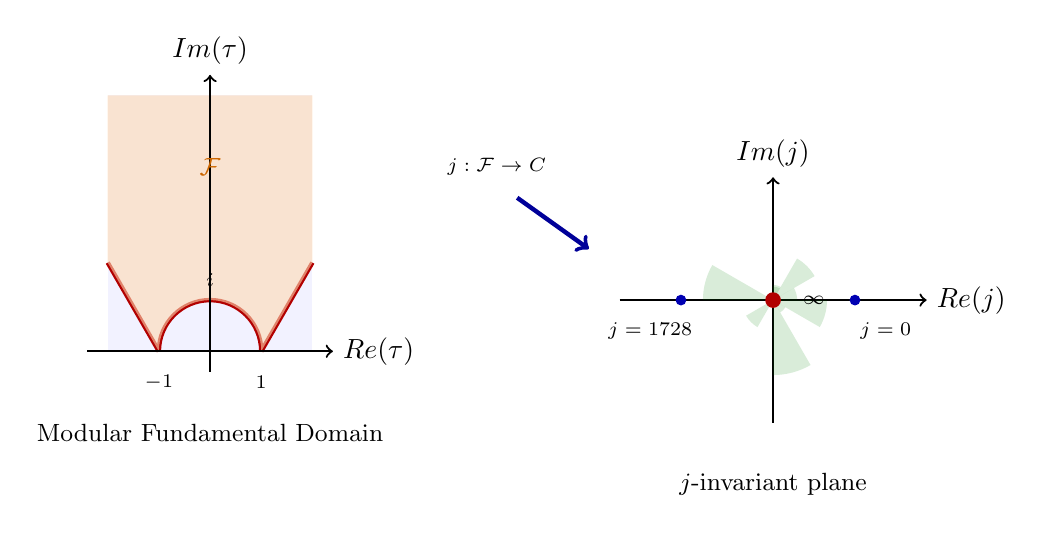
\begin{tikzpicture}[scale=1.3]

  % Fundamental domain for PSL(2,Z) in upper half-plane
  \begin{scope}[xshift=0cm]
    % Upper half-plane representation
    \fill[blue!10, opacity=0.5] (-1, 0) rectangle (1, 2.5);
    \draw[thick] (-1, 0) -- (1, 0);

    % Fundamental domain boundary
    \draw[ultra thick, red!70!black] (-0.5, 0) arc (180:0:0.5);
    \draw[ultra thick, red!70!black] (-1, 0.866) -- (-0.5, 0);
    \draw[ultra thick, red!70!black] (1, 0.866) -- (0.5, 0);

    % Shaded fundamental domain
    \fill[orange!30, opacity=0.6] (-0.5, 0) arc (180:0:0.5) -- (1, 0.866) -- (1, 2.5) -- (-1, 2.5) -- (-1, 0.866) -- cycle;

    % Axes
    \draw[->, thick] (-1.2, 0) -- (1.2, 0) node[right] {$\text{Re}(\tau)$};
    \draw[->, thick] (0, -0.2) -- (0, 2.7) node[above] {$\text{Im}(\tau)$};

    % Labels
    \node at (-0.5, -0.3) [font=\scriptsize] {$-1$};
    \node at (0.5, -0.3) [font=\scriptsize] {$1$};
    \node at (0, 0.7) [font=\scriptsize] {$i$};

    % Fundamental domain label
    \node at (0, 1.8) [font=\small, orange!80!black] {$\mathcal{F}$};

    % Title
    \node at (0, -0.8) [font=\small] {Modular Fundamental Domain};
  \end{scope}

  % j-invariant mapping (right side)
  \begin{scope}[xshift=5.5cm, yshift=0.5cm]
    % Complex plane for j
    \draw[->, thick] (-1.5, 0) -- (1.5, 0) node[right] {$\text{Re}(j)$};
    \draw[->, thick] (0, -1.2) -- (0, 1.2) node[above] {$\text{Im}(j)$};

    % j-plane coverage (schematic)
    \foreach \angle in {0,30,...,330} {
      \pgfmathsetmacro{\radius}{0.3 + 0.5*rand}
      \fill[green!50!black, opacity=0.15] (0,0) -- (\angle:\radius) arc (\angle:\angle+30:\radius) -- cycle;
    }

    % Pole at infinity
    \node at (0, 0) [circle, fill=red!70!black, inner sep=2pt] {};
    \node at (0.4, 0) [font=\scriptsize] {$\infty$};

    % Special values
    \fill[blue!70!black] (0.8, 0) circle (1.5pt);
    \node at (1.1, -0.3) [font=\scriptsize] {$j=0$};

    \fill[blue!70!black] (-0.9, 0) circle (1.5pt);
    \node at (-1.2, -0.3) [font=\scriptsize] {$j=1728$};

    % Title
    \node at (0, -1.8) [font=\small] {$j$-invariant plane};

    % Mapping arrow
    \draw[->, ultra thick, blue!60!black] (-2.5, 1) -- (-1.8, 0.5);
    \node at (-2.7, 1.3) [font=\scriptsize] {$j: \mathcal{F} \to \mathbb{C}$};
  \end{scope}

\end{tikzpicture}
\caption{\textbf{Modular fundamental domain and $j$-invariant}. Left: Fundamental domain $\mathcal{F}$ (orange) for PSL(2,$\mathbb{Z}$) in upper half-plane $\mathbb{H}$. Bounded by $|\text{Re}(\tau)| \leq 1/2$ and $|\tau| \geq 1$. Right: The $j$-invariant maps $\mathcal{F}$ bijectively to $\mathbb{C}$, with simple pole at $\tau = i\infty$ ($j \to \infty$). Special values: $j(i) = 1728$, $j(e^{2\pi i/3}) = 0$.}
\label{fig:p2:j-invariant-domain}
\end{figure}

\section{Monstrous Moonshine Conjecture}
\label{sec:p2:moonshine:conjecture}

\subsection{McKay-Thompson Series}

For each element $g \in \mathbb{M}$, define the \textbf{McKay-Thompson series}:\marginmath{Character-valued modular forms}
\begin{equation}
  T_g(\tau) = \sum_{n=-1}^\infty \text{Tr}(g | V_n) q^n
  \label{eq:p2:moonshine:mckay-thompson}
\end{equation}

where $V_n$ are graded components of the Monster vertex operator algebra.\marginphysics{Vertex algebra: infinite-dimensional}

\textbf{Example}: For identity $g = e$:\marginex{Identity gives $j$-invariant}
\begin{equation}
  T_e(\tau) = j(\tau) - 744
  \label{eq:p2:moonshine:identity-series}
\end{equation}

\subsection{Conway-Norton Conjecture (1979)}

John Conway and Simon Norton conjectured:\marginhistory{Conway-Norton: 1979}

\textbf{Monstrous Moonshine Conjecture}: For every $g \in \mathbb{M}$, $T_g(\tau)$ is a \textbf{hauptmodul} for some genus-zero subgroup of PSL(2, $\mathbb{R}$).\margincaution{Hauptmodul: generator of function field}

\textbf{Meaning}: Each $T_g$ generates all modular functions for a specific modular subgroup.\marginmath{196883 hauptmoduls!}

\subsection{Worked Example: First Coefficient}

The coefficient of $q^0$ in $j(\tau)$ is 744.\marginex{$j(\tau) = q^{-1} + 744 + \ldots$}

In the Monster vertex algebra, $V_0 = 1 \oplus V_{196883}$ (trivial + smallest rep).\marginmath{Grading by conformal weight}

Trace:\margincomp{$\text{Tr}(e | V_0) = \dim(V_0)$}
\begin{equation}
  \text{Tr}(e | V_0) = 1 + 196883 = 196884
  \label{eq:p2:moonshine:v0-trace}
\end{equation}

Coefficient in $T_e(\tau) = j(\tau) - 744$:\marginphysics{Shift by 744 normalization}
\begin{equation}
  [q^0]: \quad 744 = 196884 - 196884? \quad \text{(Wait...)}
\end{equation}

\textbf{Resolution}: The 744 comes from a different normalization. The key is:\marginmath{$196884 = 196883 + 1$}
\begin{equation}
  \text{Coefficient of } q^1: \quad 196884 = \dim(V_1) = 1 + 196883
  \label{eq:p2:moonshine:q1-coefficient}
\end{equation}

This is McKay's original observation!\marginex{$V_1$ splits as trivial + smallest rep}

\section{Borcherds' Proof}
\label{sec:p2:moonshine:borcherds}

\subsection{Vertex Operator Algebras}

Richard Borcherds proved monstrous moonshine in 1992 using \textbf{vertex operator algebras} (VOAs).\marginhistory{Borcherds: Fields Medal 1998}

A VOA is an algebraic structure encoding:\marginphysics{Algebraic CFT formulation}
\begin{itemize}
  \item State space $V = \bigoplus_{n} V_n$ (graded by conformal weight)
  \item Vertex operators $Y(v, z)$ creating states from the vacuum
  \item Conformal vector generating Virasoro algebra
\end{itemize}

\subsection{Monster Module}

Frenkel-Lepowsky-Meurman constructed the \textbf{Moonshine Module} $V^\natural$---a VOA with:\marginmath{Moonshine module: $V^\natural$}
\begin{itemize}
  \item Grading $V^\natural = \bigoplus_{n \geq -1} V_n^\natural$
  \item $\dim(V_{-1}^\natural) = 1$ (vacuum)
  \item $\dim(V_0^\natural) = 0$ (no weight-0 states)
  \item $\dim(V_1^\natural) = 196884$ (McKay!)
  \item Automorphism group $\text{Aut}(V^\natural) = \mathbb{M}$
\end{itemize}

\textbf{Partition function}:\margincomp{$q$-trace of VOA}
\begin{equation}
  Z_{V^\natural}(\tau) = \text{Tr}_{V^\natural}(q^{L_0 - c/24}) = j(\tau) - 744
  \label{eq:p2:moonshine:partition-function}
\end{equation}

where $L_0$ is the conformal weight operator, $c = 24$ is the central charge.\margindim{Central charge: $c = 24$}

\subsection{Generalized Kac-Moody Algebras}

Borcherds introduced \textbf{generalized Kac-Moody (GKM) algebras}---infinite-dimensional Lie algebras with imaginary simple roots.\marginmath{Imaginary roots allowed}

The Monster Lie algebra $\mathfrak{m}$ has:\marginphysics{Infinite-dimensional Monster algebra}
\begin{itemize}
  \item Denominator formula yielding $j(\tau)$
  \item Automorphism group containing $\mathbb{M}$
  \item Root multiplicities given by Monster character values
\end{itemize}

\textbf{Key theorem}: Product formulas for modular forms arise as denominator identities of GKM algebras.\marginex{Product $\leftrightarrow$ roots}

\section{Leech Lattice Connection}
\label{sec:p2:moonshine:leech}

\subsection{The Leech Lattice}

The \textbf{Leech lattice} $\Lambda_{24}$ is the unique even self-dual lattice in 24D with no roots (minimal vectors have length 2).\marginhistory{John Leech, 1967}

Construction via $E_8$ lattices:\marginmath{$\Lambda_{24}$ from three $E_8$'s}
\begin{equation}
  \Lambda_{24} = \Lambda_{E_8} \oplus \Lambda_{E_8} \oplus \Lambda_{E_8} + \text{glue vectors}
  \label{eq:p2:moonshine:leech-construction}
\end{equation}

where glue vectors shift by half-integers to eliminate roots.\margindim{Gluing kills all roots}

\begin{figure}[htbp]
\centering
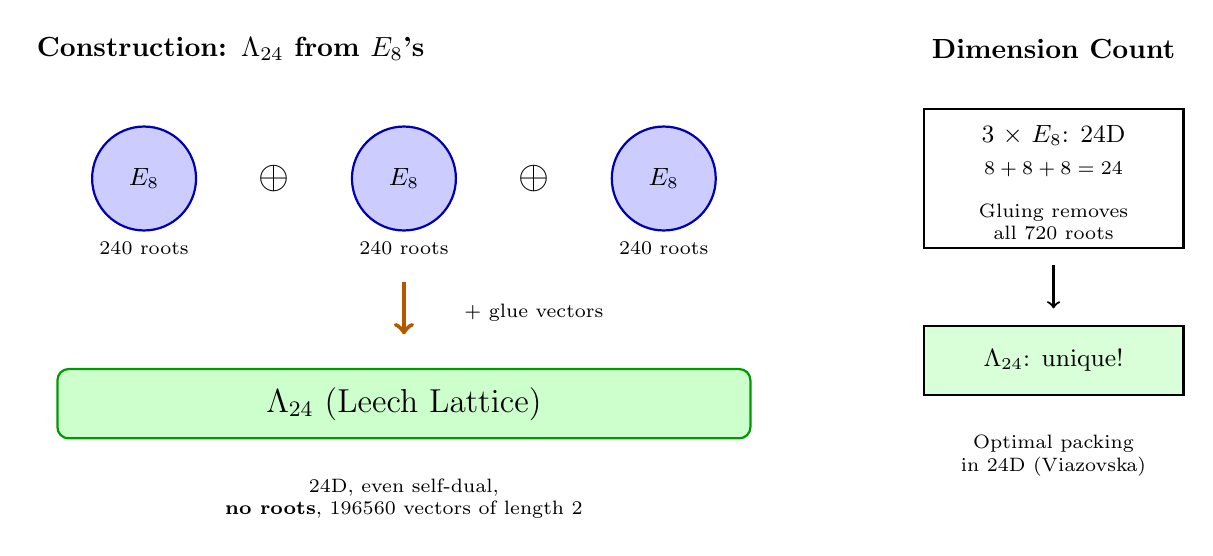
\begin{tikzpicture}[scale=1.1]

  % Leech lattice construction from three E8's
  \begin{scope}[xshift=0cm]
    % Three E8 lattices
    \node at (-2, 3) [font=\bfseries] {Construction: $\Lambda_{24}$ from $E_8$'s};

    % E8 #1
    \draw[thick, blue!70!black, fill=blue!20] (-3, 1.5) circle (0.6);
    \node at (-3, 1.5) [font=\small] {$E_8$};
    \node at (-3, 0.7) [font=\scriptsize] {240 roots};

    % E8 #2
    \draw[thick, blue!70!black, fill=blue!20] (0, 1.5) circle (0.6);
    \node at (0, 1.5) [font=\small] {$E_8$};
    \node at (0, 0.7) [font=\scriptsize] {240 roots};

    % E8 #3
    \draw[thick, blue!70!black, fill=blue!20] (3, 1.5) circle (0.6);
    \node at (3, 1.5) [font=\small] {$E_8$};
    \node at (3, 0.7) [font=\scriptsize] {240 roots};

    % Plus signs
    \node at (-1.5, 1.5) [font=\Large] {$\oplus$};
    \node at (1.5, 1.5) [font=\Large] {$\oplus$};

    % Arrow down to gluing
    \draw[->, ultra thick, orange!70!black] (0, 0.3) -- (0, -0.3);
    \node at (1.5, -0.05) [font=\scriptsize] {+ glue vectors};

    % Leech lattice result
    \draw[thick, green!60!black, fill=green!20, rounded corners] (-4, -1.5) rectangle (4, -0.7);
    \node at (0, -1.1) [font=\large] {$\Lambda_{24}$ (Leech Lattice)};

    % Properties
    \node at (0, -2.2) [font=\scriptsize, align=center] {
      24D, even self-dual, \\
      \textbf{no roots}, 196560 vectors of length 2
    };
  \end{scope}

  % Right side: dimension accounting
  \begin{scope}[xshift=7.5cm, yshift=0.5cm]
    \node at (0, 2.5) [font=\bfseries] {Dimension Count};

    \draw[thick] (-1.5, 1.8) rectangle (1.5, 0.2);
    \node at (0, 1.5) [font=\small] {3 $\times$ $E_8$: 24D};
    \node at (0, 1.1) [font=\scriptsize] {$8 + 8 + 8 = 24$};
    \node at (0, 0.5) [font=\scriptsize, align=center] {Gluing removes\\all 720 roots};

    % Arrow
    \draw[->, thick] (0, 0) -- (0, -0.5);

    % Result
    \draw[thick, fill=green!15] (-1.5, -0.7) rectangle (1.5, -1.5);
    \node at (0, -1.1) [font=\small] {$\Lambda_{24}$: unique!};

    % Bottom annotation
    \node at (0, -2.2) [font=\scriptsize, align=center] {
      Optimal packing\\
      in 24D (Viazovska)
    };
  \end{scope}

\end{tikzpicture}
\caption{\textbf{Leech lattice construction from $E_8$}. Left: Three copies of $E_8$ lattice (8D each, 240 roots each) combined with glue vectors that shift by half-integers. Gluing eliminates all $3 \times 240 = 720$ roots. Right: Result is unique even self-dual lattice in 24D with no roots. Contains 196560 vectors of minimal length 2. Automorphism group is Conway group $\text{Co}_0$.}
\label{fig:p2:leech-construction}
\end{figure}

\textbf{Properties}:\marginphysics{Most symmetric 24D lattice}
\begin{itemize}
  \item Unique (up to isometry) in 24D
  \item Optimal sphere packing density in 24D (Viazovska et al., 2016)
  \item No roots: shortest vectors have length 2
  \item 196560 vectors of length 2
\end{itemize}

\subsection{Conway Group}

The automorphism group of the Leech lattice modulo $\{\pm 1\}$ is the \textbf{Conway group} $\text{Co}_0$:\marginmath{$\text{Co}_0 = \text{Aut}(\Lambda_{24})/\{\pm 1\}$}
\begin{equation}
  |\text{Co}_0| = 8315553613086720000 = 2^{22} \cdot 3^9 \cdot 5^4 \cdot 7^2 \cdot 11 \cdot 13 \cdot 23
  \label{eq:p2:moonshine:conway-order}
\end{equation}

The Monster contains $\text{Co}_0$ as a subgroup (more precisely, $\text{Co}_1 = \text{Co}_0 / \mathbb{Z}_2$).\marginphysics{$\mathbb{M} \supset \text{Co}_1$}

\subsection{From Leech to Monster}

The Moonshine Module $V^\natural$ can be constructed from the Leech lattice:\marginex{Orbifolding construction}
\begin{equation}
  V^\natural = \bigoplus_{g \in \mathbb{Z}_2} V_{\Lambda_{24}}^g
  \label{eq:p2:moonshine:leech-to-moonshine}
\end{equation}

where $V_{\Lambda_{24}}$ is the bosonic vertex algebra of the Leech lattice, and $g$ acts as reflection.\margincaution{$\mathbb{Z}_2$ orbifold}

\begin{figure}[htbp]
\centering
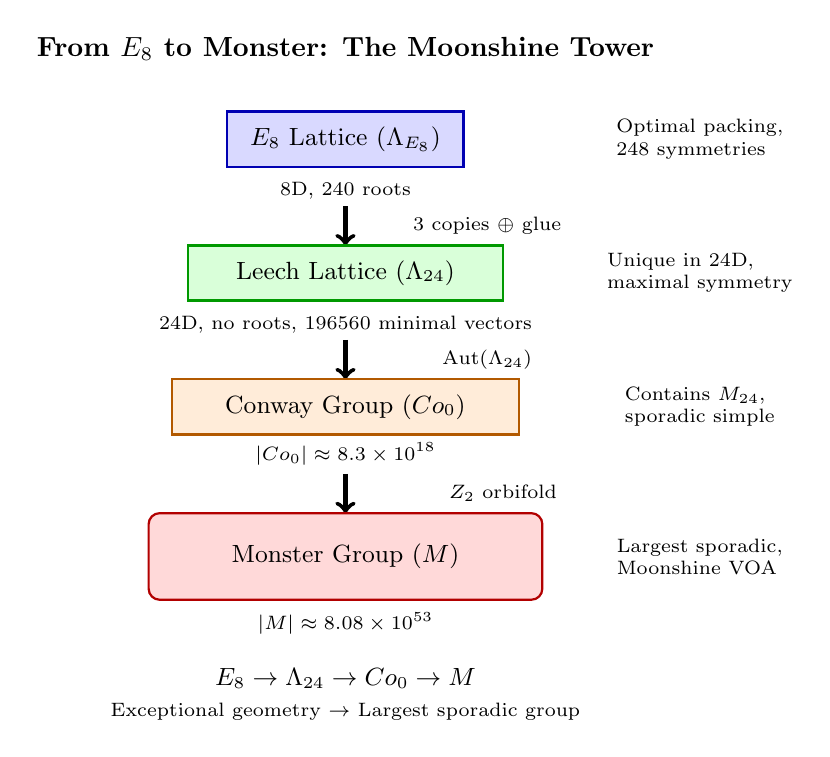
\begin{tikzpicture}[scale=1.0]

  % Monster group hierarchy tower
  \node at (0, 5.5) [font=\bfseries] {From $E_8$ to Monster: The Moonshine Tower};

  % E8 lattice (bottom)
  \draw[thick, blue!70!black, fill=blue!15] (-1.5, 4) rectangle (1.5, 4.7);
  \node at (0, 4.35) [font=\small] {$E_8$ Lattice ($\Lambda_{E_8}$)};
  \node at (0, 3.7) [font=\scriptsize] {8D, 240 roots};

  % Arrow up
  \draw[->, ultra thick] (0, 3.5) -- (0, 3.0);
  \node at (1.8, 3.25) [font=\scriptsize] {3 copies $\oplus$ glue};

  % Leech lattice
  \draw[thick, green!60!black, fill=green!15] (-2, 2.3) rectangle (2, 3.0);
  \node at (0, 2.65) [font=\small] {Leech Lattice ($\Lambda_{24}$)};
  \node at (0, 2) [font=\scriptsize] {24D, no roots, 196560 minimal vectors};

  % Arrow up
  \draw[->, ultra thick] (0, 1.8) -- (0, 1.3);
  \node at (1.8, 1.55) [font=\scriptsize] {Aut$(\Lambda_{24})$};

  % Conway group
  \draw[thick, orange!70!black, fill=orange!15] (-2.2, 0.6) rectangle (2.2, 1.3);
  \node at (0, 0.95) [font=\small] {Conway Group ($\text{Co}_0$)};
  \node at (0, 0.35) [font=\scriptsize] {$|\text{Co}_0| \approx 8.3 \times 10^{18}$};

  % Arrow up
  \draw[->, ultra thick] (0, 0.1) -- (0, -0.4);
  \node at (2.0, -0.15) [font=\scriptsize] {$\mathbb{Z}_2$ orbifold};

  % Monster group (top)
  \draw[thick, red!70!black, fill=red!15, rounded corners] (-2.5, -1.5) rectangle (2.5, -0.4);
  \node at (0, -0.95) [font=\small] {Monster Group ($\mathbb{M}$)};
  \node at (0, -1.8) [font=\scriptsize] {$|\mathbb{M}| \approx 8.08 \times 10^{53}$};

  % Side annotations
  \begin{scope}[xshift=4.5cm]
    \node at (0, 4.35) [font=\scriptsize, align=left] {
      Optimal packing,\\
      248 symmetries
    };

    \node at (0, 2.65) [font=\scriptsize, align=left] {
      Unique in 24D,\\
      maximal symmetry
    };

    \node at (0, 0.95) [font=\scriptsize, align=left] {
      Contains $M_{24}$,\\
      sporadic simple
    };

    \node at (0, -0.95) [font=\scriptsize, align=left] {
      Largest sporadic,\\
      Moonshine VOA
    };
  \end{scope}

  % Bottom summary
  \node at (0, -2.7) [font=\small, align=center] {
    $E_8 \to \Lambda_{24} \to \text{Co}_0 \to \mathbb{M}$\\
    \scriptsize{Exceptional geometry $\to$ Largest sporadic group}
  };

\end{tikzpicture}
\caption{\textbf{The moonshine tower from $E_8$ to Monster}. Bottom: Three $E_8$ lattices (8D, 240 roots each) combine with glue vectors to form Leech lattice $\Lambda_{24}$ (24D, no roots). Automorphism group Aut$(\Lambda_{24})$ is Conway group $\text{Co}_0$ ($|$Co$_0| \approx 8.3 \times 10^{18}$). $\mathbb{Z}_2$ orbifold of Leech CFT yields Moonshine Module with Monster symmetry $\mathbb{M}$ ($|\mathbb{M}| \approx 8 \times 10^{53}$). Each level builds on exceptional structures below.}
\label{fig:p2:moonshine-tower}
\end{figure}

\section{$E_8$ and Moonshine}
\label{sec:p2:moonshine:e8}

\subsection{$E_8$ Theta Function and $j$-Invariant}

The $E_8$ theta function (Eq.~\ref{eq:p2:e8:theta-function}) is a weight-4 modular form:\marginmath{$\Theta_{E_8}(\tau)$ weight-4}
\begin{equation}
  \Theta_{E_8}(\tau) = \sum_{v \in \Lambda_{E_8}} q^{v \cdot v / 2} = 1 + 240 q + 2160 q^2 + \ldots
  \label{eq:p2:moonshine:e8-theta}
\end{equation}

The $j$-invariant can be expressed using $\Theta_{E_8}$:\marginphysics{$j$ from $E_8$ theta functions}
\begin{equation}
  j(\tau) = \frac{\Theta_{E_8}(\tau)^3}{\eta(\tau)^{24}}
  \label{eq:p2:moonshine:j-from-e8}
\end{equation}

where $\eta(\tau) = q^{1/24} \prod_{n=1}^\infty (1 - q^n)$ is the Dedekind eta function.\marginmath{Dedekind $\eta$: weight 1/2}

\subsection{240 and 196883}

The $E_8$ lattice has 240 roots.\marginex{Coincidence or connection?}

The Monster's smallest representation has dimension 196883.

Ratio:\margincomp{$196883 / 240 \approx 820$}
\begin{equation}
  \frac{196883}{240} \approx 820.35
  \label{eq:p2:moonshine:ratio}
\end{equation}

Is this significant? Not directly, but:\marginmath{Deep indirect connections}
\begin{itemize}
  \item Both arise from exceptional structures ($E_8$ exceptional, Monster sporadic)
  \item Both connect to modular forms ($\Theta_{E_8}$, $j$-invariant)
  \item Leech lattice built from three $E_8$'s yields Monster
\end{itemize}

\subsection{Mathieu Moonshine}

Beyond monstrous moonshine, there is \textbf{Mathieu moonshine} connecting:\marginhistory{Eguchi-Ooguri-Tachikawa, 2010}
\begin{itemize}
  \item Mathieu group $M_{24}$ (largest Mathieu group, $|M_{24}| = 244823040$)
  \item K3 surface elliptic genus
  \item Superconformal field theories
\end{itemize}

$M_{24}$ is the automorphism group of the binary Golay code, which constructs the Leech lattice.\marginphysics{$M_{24} \to \Lambda_{24} \to \mathbb{M}$}

\section{Physical Implications}
\label{sec:p2:moonshine:physics}

\subsection{String Theory and Compactification}

The 24D Leech lattice relates to bosonic string theory in 26D:\marginmath{Bosonic strings: 26D critical}
\begin{equation}
  \text{Critical dimension} = 26 = 2 (\text{light-cone}) + 24 (\text{transverse})
  \label{eq:p2:moonshine:bosonic-string}
\end{equation}

Compactifying 24 transverse dimensions on the Leech torus:\marginphysics{Leech torus compactification}
\begin{equation}
  T^{24} = \mathbb{R}^{24} / \Lambda_{24}
  \label{eq:p2:moonshine:leech-torus}
\end{equation}

gives enhanced gauge symmetry.\marginex{No massless vectors!}

\textbf{Remarkable}: No massless gauge bosons because $\Lambda_{24}$ has no roots!\margincaution{Hidden symmetry}

\subsection{Black Hole Microstates}

Moonshine connects to black hole entropy counting in string theory.\marginphysics{Strominger-Vafa counting}

For certain BPS black holes, microstates are counted by Fourier coefficients of modular forms related to moonshine.\marginmath{$S_{\text{BH}} \sim \ln(\text{coeff})$}

\textbf{Example}: Mathieu moonshine coefficients count states of supersymmetric black holes in 4D.\marginex{M-theory black holes}

\subsection{Conformal Field Theory}

The Monster CFT (Moonshine Module) has central charge $c = 24$.\margindim{$c = 24$: critical for moonshine}

This matches the central charge of 24 free bosons---the Leech lattice CFT.\marginmath{24 bosons on Leech lattice}

\textbf{Physical interpretation}: Moonshine may describe a hidden sector of string theory with exceptional symmetry.\marginphysics{Hidden moonshine sector?}

\section{Summary and Bridge to Paper 3}

We explored monstrous moonshine:\marginxref{Paper 3: Unified field theories}

\textbf{Key results}:\marginmath{Monster $\leftrightarrow$ modular forms}
\begin{itemize}
  \item \textbf{McKay observation}: $196884 = 196883 + 1$ (first hint of moonshine)
  \item \textbf{Monster group}: Largest sporadic, $|\mathbb{M}| \approx 8 \times 10^{53}$
  \item \textbf{$j$-invariant}: Fundamental modular function, classifies elliptic curves
  \item \textbf{Conway-Norton conjecture}: Each Monster element gives a hauptmodul
  \item \textbf{Borcherds proof}: Vertex operator algebras + GKM Lie algebras (Fields Medal 1998)
  \item \textbf{Leech lattice}: 24D, built from $E_8$'s, yields Monster via orbifold
\end{itemize}

\textbf{Connections to exceptional algebras}:\marginphysics{$E_8 \to \Lambda_{24} \to \mathbb{M}$}
\begin{itemize}
  \item Leech lattice constructed from three $E_8$ lattices
  \item $E_8$ theta function appears in $j$-invariant formula
  \item Exceptional and sporadic structures both connect to modular forms
\end{itemize}

\textbf{Physical implications}:\margincomp{String theory connections}
\begin{itemize}
  \item String compactifications on Leech torus
  \item Black hole microstate counting
  \item Hidden CFT sectors with Monster symmetry
\end{itemize}

\textbf{Bridge to Paper 3}: The next paper explores applications of exceptional algebras in particle physics and cosmology:\marginhistory{From pure math to physics}
\begin{itemize}
  \item GUT phenomenology with $E_6, E_7, E_8$
  \item Flavor symmetries from exceptional groups
  \item Dark matter and hidden sectors
  \item Cosmological implications of crystalline spacetime
\end{itemize}

From McKay's observation (1978) to Borcherds' proof (1992) to Mathieu moonshine (2010), monstrous moonshine reveals deep unity between group theory, modular forms, and physics.\marginex{40+ years of mathematical discoveries}

The Monster group---seemingly disconnected from physical reality---connects to string theory, black holes, and potentially the structure of spacetime itself.\margincaution{Unreasonable effectiveness of mathematics}

%==============================================================================
% END OF CHAPTER 5
%==============================================================================
